% ==============================================================================
% APRESENTAÇÃO DE DEFESA DE TCC — INSTITUTO FEDERAL DE SERGIPE (IFS)
% Formato Widescreen 16:9 | 100% compatível com pdflatex
% Reutiliza automaticamente ../src/referencias.bib e ../src/figuras/
%
% Compilação recomendada (na raiz do projeto):
%   Windows:   .\make.bat slides
%   Linux/Mac: make slides
% ==============================================================================
\documentclass[aspectratio=169, 11pt]{beamer}

\usepackage[utf8]{inputenc}
\usepackage[T1]{fontenc}
\usepackage[brazil]{babel}
\usepackage{lmodern}
\usepackage{csquotes}
\usepackage{graphicx}
\usepackage{booktabs}

% Tema Institucional do IFS (slides/tema-ifs.sty)
\usepackage{tema-ifs}

% Reaproveita automaticamente todas as figuras e diagramas do TCC (zero duplicação)
\graphicspath{{../src/figuras/}{../src/figuras/diagramas/}{../src/figuras/graficos/}{../src/figuras/capturas/}{../src/}}

% Reaproveita a mesma base bibliográfica do TCC no padrão ABNT
\usepackage[backend=biber, style=abnt]{biblatex}
\addbibresource{../src/referencias.bib}
\setbeamertemplate{bibliography item}{}

% ==============================================================================
% METADADOS DA APRESENTAÇÃO (Alinhe com src/metadados.tex)
% ==============================================================================
\title[RAG e MCP — Defesa de TCC]{Avaliação Experimental de Arquiteturas Baseadas em RAG e MCP}
\subtitle{Trabalho de Conclusão de Curso — Bacharelado em Sistemas de Informação}
\author[José Gustavo C. Nascimento]{José Gustavo Correia Nascimento \\[4pt] {\footnotesize\normalfont Orientação: Prof. Diego Armando}}
\institute{INSTITUTO FEDERAL DE SERGIPE — CAMPUS LAGARTO}
\date{Lagarto -- SE, 2026}

% Exibe slide de transição suave no início de cada seção (comente se preferir pular)
\AtBeginSection[]{\ifssectionframe}

\begin{document}

% ==============================================================================
% 1. CAPA INSTITUCIONAL
% ==============================================================================
\begin{frame}[plain]
  \titlepage
\end{frame}

% ==============================================================================
% 2. ROTEIRO DA APRESENTAÇÃO
% ==============================================================================
\begin{frame}{Roteiro da Apresentação}
  \tableofcontents
\end{frame}

% ==============================================================================
% 3. INTRODUÇÃO
% ==============================================================================
\section{Introdução e Objetivos}

\begin{frame}{Contextualização e Problema de Pesquisa}
  \framesubtitle{Por que este problema é relevante para a Engenharia de Software e IA?}
  \begin{columns}[T, onlytextwidth]
    \begin{column}{0.52\textwidth}
      \begin{block}{Contexto}
        A adoção de fluxos reprodutíveis e arquiteturas modulares eleva a confiabilidade de sistemas baseados em conhecimento~\cite{exemplo2026}.
      \end{block}
      \vspace{0.25cm}
      \begin{itemize}
        \item Ambientes padronizados reduzem falhas de integração~\cite{devcontainer}.
        \item Necessidade de métricas objetivas para comparar arquiteturas.
      \end{itemize}
    \end{column}
    \begin{column}{0.44\textwidth}
      \begin{alertblock}{Problema de Pesquisa}
        Como avaliar experimentalmente, de forma reproduzível e auditável, o desempenho de arquiteturas baseadas em RAG e MCP sob restrições reais?
      \end{alertblock}
    \end{column}
  \end{columns}
\end{frame}

\begin{frame}{Objetivos da Pesquisa}
  \begin{block}{Objetivo Geral}
    Avaliar experimentalmente arquiteturas baseadas em RAG e MCP, estabelecendo critérios quantitativos e qualitativos de precisão, latência e rastreabilidade.
  \end{block}
  \vspace{0.3cm}
  \textbf{\color{IFSVerde}Objetivos Específicos:}
  \begin{enumerate}
    \item Mapear a fundamentação teórica e os requisitos arquiteturais da literatura.
    \item Projetar e implementar o ambiente experimental reprodutível.
    \item Conduzir experimentos controlados com coleta sistemática de métricas.
    \item Analisar comparativamente os resultados e documentar recomendações práticas.
  \end{enumerate}
\end{frame}

% ==============================================================================
% 4. METODOLOGIA
% ==============================================================================
\section{Metodologia e Arquitetura}

\begin{frame}{Arquitetura e Fluxo Metodológico}
  \framesubtitle{Diagrama reutilizado diretamente de \texttt{src/figuras/exemplo-diagrama.pdf}}
  \centering
  \IfFileExists{../src/figuras/exemplo-diagrama.pdf}{%
    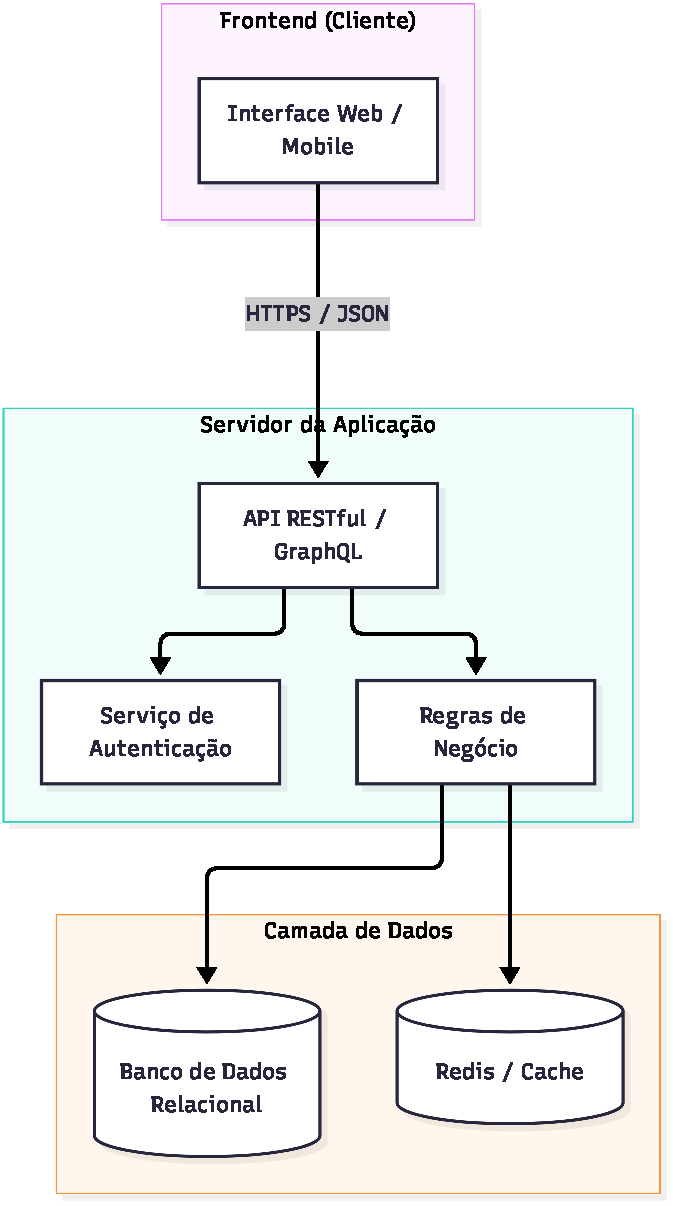
\includegraphics[width=0.78\textwidth, height=0.62\textheight, keepaspectratio]{exemplo-diagrama.pdf}
  }{%
    \begin{exampleblock}{Espaço reservado para figura}
      Execute \texttt{make figures} para gerar o diagrama vetorial em \texttt{src/figuras/}.
    \end{exampleblock}
  }
  \par\vspace{0.2cm}
  {\scriptsize\color{IFSCinzaTexto}Fonte: Elaborado pelo autor (2026).}
\end{frame}

% ==============================================================================
% 5. RESULTADOS E DISCUSSÃO
% ==============================================================================
\section{Resultados e Discussão}

\begin{frame}{Principais Resultados Obtidos}
  \framesubtitle{Síntese quantitativa dos experimentos (substitua pelos dados finais do TCC)}
  \begin{columns}[T, onlytextwidth]
    \begin{column}{0.31\textwidth}
      \metriccard{94,2\%}{Acurácia Média na Validação}
    \end{column}
    \begin{column}{0.31\textwidth}
      \metriccard{--38\%}{Redução no Tempo de Resposta}
    \end{column}
    \begin{column}{0.31\textwidth}
      \metriccard{100\%}{Reprodutibilidade dos Testes}
    \end{column}
  \end{columns}

  \vspace{0.5cm}
  \centering
  \small
  \begin{tabular}{@{}lccc@{}}
    \toprule
    \textbf{Arquitetura} & \textbf{Precisão (\%)} & \textbf{Latência (ms)} & \textbf{Cobertura (\%)} \\
    \midrule
    Baseline (Consulta Direta) & 78,4 & 420 & 81,0 \\
    RAG Convencional           & 88,9 & 610 & 92,5 \\
    \textbf{RAG + MCP (Proposta)} & \textbf{94,2} & \textbf{380} & \textbf{97,8} \\
    \bottomrule
  \end{tabular}
\end{frame}

% ==============================================================================
% 6. CONCLUSÃO
% ==============================================================================
\section{Conclusão e Trabalhos Futuros}

\begin{frame}{Considerações Finais}
  \begin{columns}[T, onlytextwidth]
    \begin{column}{0.48\textwidth}
      \begin{block}{Principais Contribuições}
        \begin{itemize}
          \item Validação experimental comparativa entre arquiteturas.
          \item Protocolo reproduzível de avaliação e auditoria.
          \item Base documental e ferramental aberta para novos estudos.
        \end{itemize}
      \end{block}
    \end{column}
    \begin{column}{0.48\textwidth}
      \begin{exampleblock}{Trabalhos Futuros}
        \begin{itemize}
          \item Expansão da base experimental para novos domínios.
          \item Avaliação com modelos locais de menor custo computacional.
          \item Integração contínua em ambiente produtivo institucional.
        \end{itemize}
      \end{exampleblock}
    \end{column}
  \end{columns}
\end{frame}

% ==============================================================================
% 7. REFERÊNCIAS (EXTRAÍDAS DE ../src/referencias.bib)
% ==============================================================================
\begin{frame}[allowframebreaks]{Referências}
  \printbibliography[heading=none]
\end{frame}

% ==============================================================================
% 8. ENCERRAMENTO / BANCA EXAMINADORA
% ==============================================================================
\begin{frame}[plain]
  \begin{tikzpicture}[remember picture, overlay]
    \fill[IFSGrafite] (current page.south west) rectangle (current page.north east);
    \fill[IFSVerde] (current page.south west) rectangle ([xshift=0.55cm]current page.north west);
  \end{tikzpicture}
  \vfill
  \centering
  {\Huge\bfseries\color{IFSFundo}Obrigado!\par}
  \vspace{0.35cm}
  {\large\color{IFSVerdeClaro}Perguntas e Considerações da Banca Examinadora\par}
  \vspace{0.6cm}
  \begin{tikzpicture}\fill[IFSVerdeClaro] (0,0) rectangle (3.5cm, 2pt);\end{tikzpicture}
  \vspace{0.45cm}
  {\normalsize\color{IFSFundo}\textbf{José Gustavo Correia Nascimento}\par}
  \vspace{0.15cm}
  {\footnotesize\color{IFSCinzaClaro}Bacharelado em Sistemas de Informação — IFS Campus Lagarto\par}
  \vfill
\end{frame}

\end{document}
